\documentclass[12pt,letterpaper]{article}

%\usepackage{fontspec}
%\usepackage[utf8]{inputenc}
\usepackage{textcomp,marvosym}
\usepackage{amsmath,amssymb}
\usepackage[left]{lineno}
\usepackage{changepage}
\usepackage{rotating}
\usepackage{natbib}
\usepackage{setspace} 
\usepackage{lastpage}
\usepackage{fancyhdr}
\usepackage{graphicx}
\usepackage{wrapfig}
\usepackage{hyperref}
\usepackage{float}
\usepackage[small]{titlesec}
\usepackage[font=small,labelfont=bf, labelsep=period]{caption}
\usepackage{booktabs}
%\doublespacing

%\raggedright
\textwidth = 6.5 in
\textheight = 8.0 in
\oddsidemargin = 0.0 in
\evensidemargin = 0.0 in
\topmargin = 0.0 in
\headheight = 0.0 in
\headsep = 0.5 in
\parskip = 0.05 in
\parindent = 0.1in

% Bold the 'Figure #' in the caption and separate it from the title/caption with a period
% Captions will be left justified
%\usepackage[aboveskip=1pt,labelfont=bf,labelsep=period,justification=raggedright,singlelinecheck=off]{caption}

% Remove brackets from numbering in List of References
%\makeatletter
%\renewcommand{\@biblabel}[1]{\quad#1.}
%\makeatother

\pagestyle{myheadings}
\pagestyle{fancy}
\fancyhf{}
\lhead{Fairchild} 
\chead{\textit{Investigating the geomagnetic signature of inner core growth}}
\rhead{\thepage/\pageref{LastPage}}

%\renewenvironment{abstract}
% {\small
%  \begin{center}
%  \bfseries \abstractname\vspace{-.5em}\vspace{0pt}
%  \end{center}
%  \list{}{
%    \setlength{\leftmargin}{.5cm}%
%    \setlength{\rightmargin}{\leftmargin}%
%  }%
%  \item\relax}
% {\endlist}


%\documentclass[12pt,a4paper]{article}
\usepackage[a4paper, margin=0.75in]{geometry}
\usepackage{siunitx}
\usepackage{textcomp}

\titlespacing*{\section}
{0pt}{5pt}{0pt}
\titlespacing*{\subsection}
{0pt}{0pt}{0pt}

\begin{document}
\begin{flushleft}
{\large \textbf{Investigating the geomagnetic signature of inner core growth using the Calypso geodynamo model}}\\
\vspace{0.3em}
Luke Fairchild, EPS 236 Term Paper --- 12/14/2016
%Luke M. Fairchild\textsuperscript{1,2},
%Nicholas L. Swanson-Hysell\textsuperscript{1},
%Sonia M. Tikoo\textsuperscript{1,3}
%\title{Modeling the flexural and thermal subsidence of the 1.1 Ga Midcontinent Rift}
%\author{Luke Fairchild}
%\begin{document}
%\maketitle{}
\end{flushleft}

\section*{Introduction}
Earth's magnetic field is generated by fluid motion within the liquid outer core. This fluid motion of the geodynamo is sustained by both thermal and compositional convection. The relative importance of these two modes of convection in powering the geodynamo is determined by the thermal evolution of the core and the eventual nucleation and growth of the solid inner core. At present estimates for the core-mantle boundary (CMB) heat flux and the inner core radius, analytical models indicate that approximately two thirds of the ohmic dissipation in the core owes to compositional convection and one third to thermal convection \citep{Buffett1996a}. On the other hand, evidence for an active geodynamo as early at 3.4 Ga \citep{Tarduno2007a}---when the CMB heat flux was much greater and the core entirely liquid---suggests that the early geodynamo was likely powered entirely by thermal convection. The nucleation of the solid inner core marks the onset of compositional convection and therefore a major transitioning of the geodynamo, as the freezing of iron at the inner core boundary releases latent heat and buoyant impurities into the liquid outer core. These two distinct convective regimes can be generally described as top-driven (powered by heat flux at the ``top'', or the CMB) and bottom-driven (powered by processes at the ``bottom'', or inner core boundary). If the transition between these two geodynamo systems can be accurately modeled, a geomagnetic signature of inner core nucleation and growth can be characterized and potentially identified within the paleomagnetic record.
%\subsection*{The geomagnetic signature of inner core nucleation}
%Outline different arguments (from Biggin2015 to Driscoll2016)
\section*{Modeling the geodynamo}
%top vs bottom driven
%\subsection*{
%\subsection*{Model parameters}
To simulate both a top- and bottom-driven dynamo, I varied the sign of the heat source value $Q_T$ (see Eq. \ref{eq:temp} below) within the geodynamo model \textit{Calypso} \citep{Matsui2014a}. The model was parameterized by the following non-dimensional values, where $Ra$ is a modified Rayleigh number, $Pr$ is the Prandtl number, $Pr_m$ is the magnetic Prandtl number, and $Ek$ is the Ekman number. 

\begin{tabular}{cccc}
\toprule
$Ra$ &  $Pr$ &  $Pr_m$ &     $Ek$ \\
\midrule
1200 &   1.0 &     1.0 &  0.00005 \\
\bottomrule
\end{tabular}



The \textit{Calypso} model performs a magnetohydrodynamics simulation within a rotating spherical shell. The governing equations solved by \textit{Calypso} include a momentum equation (magnetohydrodynamic form of the Navier-Stokes equations accounting for the addition of Lorentz and Coriolis forces) 
\begin{equation}\label{eq:momentum}
\frac{\partial \mathbf{u}}{\partial t} + (\boldsymbol{\omega}\times\mathbf{u}) = -\nabla[P+\frac{1}{2}u^2] - \nu\nabla\times\nabla\times\mathbf{u} - 2\Omega(\hat{z}\times\mathbf{u}) + \frac{\rho}{\rho_0}\mathbf{g} + \frac{1}{\rho_0}(\mathbf{J}\times\mathbf{B}),
\end{equation}
%\begin{equation}\label{eq:incompressibility}
%\nabla\cdot\mathbf{u}=0;
%\end{equation}
with the incompressibility condition, $\nabla\cdot\mathbf{u}=0$; the induction equation 
\begin{equation}\label{eq:induction}
\frac{\partial \mathbf{B}}{\partial t}=\nabla\times(\mathbf{u}\times\mathbf{B})-\eta\nabla\times\nabla\times\mathbf{B}
\end{equation}
with $\nabla\cdot\mathbf{B}=0$; and a temperature evolution equation
\begin{equation}\label{eq:temp}
\frac{\partial T}{\partial t}+(\mathbf{u}\cdot\nabla)T = \kappa_T\nabla^2T + Q_T.
\end{equation}

Further details and other governing equations of the model can be found in \cite{Matsui2014a}.


\section*{Results and Discussion}
\subsection*{Thermal regimes of the current models}
At present, I have been able to achieve two distinct thermal states of the outer core through varying the heat source term $Q_T$. These will be referred to as 1) the ``bottom-driven'' model (B.D.) and 2) the ``top- and bottom-driven'' model (T\&B.D). Model B.D. ($Q_T = -5$) is a well-developed ``heat sink'' that simulates a bottom-driven geodynamo powered by latent heat and light element release at the inner core boundary. Model T\&B.D. ($Q_T = +5$) simulates a gedynamo that is both top- and bottom-driven, representative of a balance between primitive thermal, or top-driven, convection (due to secular cooling of the core) and the thermal and compositional convection driven from the bottom (due to solidification of the inner core). For both models, the radial heat flux can be computed by $q=r^2\frac{\partial T}{\partial r}$, and the average heat flux $q*$ for both the inner core boundary and the CMB is shown in Figure \ref{fig:composite}a. While comparing these two preliminary thermal regimes still benefits the goal of this project, I have not yet achieved an entirely top-driven model representative of the early geodynamo without a solidifying inner core. However, efforts to do so are currently in progress (see \textit{Future investigations} below).

\subsection*{Structure of the geomagnetic field}
It has been argued on the basis of geodynamo models that growth of the inner core should correlate with an increase in magnetic field intensity \citep{Aubert2009a}, and such a signal may have already been identified in the Mesoproterozoic paleointensity record \citep{Biggin2015a}. In this project, I focus on the structure, rather than the intensity, of the geomagnetic field in trying to identify signatures of inner core growth. A more thorough treatment of the effect of inner core growth on field morphology can be found in \cite{Driscoll2016b}.

Model B.D. maintains a dominant, axially aligned dipole field (Fig. \ref{fig:composite}c). While fluctuations are present, as seen by the diffuse patches of magnetic flux at the CMB (Fig. \ref{fig:composite}c), the large-scale structure of the field can be organized by symmetry about the equator consistent with that of a geocentric axial dipole. The geomagnetic field can be expanded with spherical harmonics and gauss coefficients corresponding to the various $l$ and $m$ terms. In model B.D., a minimum of 99.0\% of the magnetic field can be fit using only the axial dipole gauss coefficient, $g^{0}_{1}$. 

While the magnetic field of model T\&B.D. remains similarly dominated by that of an axial dipole, deviations are much more significant. In particular, the $h^{1}_{1}$ gauss coefficient (representing an equatorial dipole field) grows to $\sim$10\% of $g^{0}_{1}$ by the end of the T\&B.D. simulation (Fig. \ref{fig:source_gauss}). It is possible that, given a longer run time (this is currently in progress), the equatorial dipole component would become even more prominent. This result is similar to the Neoproterozoic ``weak-field'' state of the geodyanmo just prior to inner core nucleation at $\sim$650 Ma proposed by \cite{Driscoll2016b}, in which non-axial dipole fields become significant. \cite{Driscoll2016b} hypothesized that such a state resulted from diminished thermal buoyancy due to secular cooling and that a strong, axial dipole field was reinstated by the compositional convection of inner core nucleation. The results of model T\&B.D. are intriguing in that they produce a similar effect regarding non-axial, dipolar field structures (but not intensity) with some combination of top- and bottom-driven convection prescribed by the model's heat source term, $Q_T=+5$. The relative magnitude of the $h^{1}_{1}$ coefficient in model T\&B.D., while still significant, is not quite as large as in the model of \cite{Driscoll2016b}. Increasing the vigor of convection---perhaps by raising $Ra$ to $5\times10^6$, as in the \cite{Driscoll2016b} model---could amplify the $h^{1}_{1}$ signal and make this comparison more robust.

\subsection*{Secular variation}
The changes in field structure as outlined above would be reflected in the secular variation of paleomagnetic poles. The magnetic field $H$ at the earth's surface can be calculated by $H=-\nabla\psi$, where $\psi$ is the magnetic potential field. We can solve for $\psi$ by using the gauss coefficients $g^{m}_{l}$ and $h^{m}_{l}$ in the spherical harmonic expansion
\begin{equation}
\psi_m(r, \theta, \phi)=\frac{a}{\mu_0}\sum_{l=1}^{\infty}\sum_{m=0}^{l}(\frac{a}{r})^{l+1}P_{l}^{m}(\cos{\theta})(g^{m}_{l}\cos{m\phi}+h^{m}_{l}\sin{m\phi})
\end{equation}
where $a$ is the radius of Earth, $\mu_0$ is the magnetic permeability of free space, $P_{l}^{m}$ are partially normalized Schmidt polynomials, $\theta$ is colatitude and $\psi$ is longitude.

Before evaluating the geomagnetic variations of the models, it is important to attempt to scale the non-dimensional time step of the geodynamo model to a real time range over which the true geodynamo operates. For both models BD and T\&BD, the non-dimensional time step is $\Delta t_{model}=5\times10^{-7}$ and diffusion time scales are simplified by setting the magnetic Prandtl number, $P_m=\frac{\nu}{\eta}$, to 1. If the shell thickness ($r_{CMB}-r_{ICB}$) is $L$, and we assume that a reasonable characteristic time scale is $\tau_{\eta}$, where $\tau_{\eta} = \frac{L^2}{\eta}$, then we can set $\eta$ to a realistic value of $1.6\ m^2/s$ and obtain $\tau_{\eta}\approx 3.19\times10^{12}$. Given $t_{real}=\tau_{\eta} t_{model}$, $2\times10^5$ time steps in the simulations (a minimum range for which both models were run) should represent $\sim10^4$ years of geodynamo operation. If these estimations are correct, the geomagnetic variations observed within the geodynamo models are comparable (in their time scale) to secular variation in paleomagnetic data.

For each model, I segmented the full run time of the simulation into 10 equal intervals; within each interval, I extracted the gauss coefficients for a randomly chosen time instant to simulate paleomagnetic data collection. I then solved for the magnetic field $H$ for each set of gauss coefficients at 0\textdegree\ N, 0\textdegree\ E and calculated their corresponding virtual geomagnetic pole (VGP) assuming a geocentric axial dipole field, as is done for most paleomagnetic directional data. 

As expected, model T\&BD shows a larger VGP scatter (Fig. \ref{fig:vgps}) owing to the greater structural complexity of the field as discussed above, whereas the simulated VGPs of model BD show virtually no scatter. In spite of this difference, there are no characteristic patterns of these distributions that would allow them to be distinguished in real paleomagnetic data. To improve the realism of these models and perhaps resolve distinct secular variation patterns, future implementations of these models could amplify fluctuations by increasing $Ra$ and the vigor of convection. 

\subsection*{Future investigations}
In an effort to better simulate an entirely top-driven geodynamo, I am currently running simulations with a heat source value of $Q_T=+10$. I also plan to implement these models with a higher $Ra$ in order to better resolve geomagnetic fluctuations and potentially amplify the non-axial dipole or multipole components of the geomagnetic field.


\begin{figure}
\centering
\includegraphics[width=\textwidth]{composite.pdf}
\caption{\small{Comparison of results from models B.D. and T\&B.D. Panel A shows the temperature profile of the core and the average heat flux at the inner core boundary ($q*_{ICB}$) and outer core boundary ($q*_{CMB}$). Panel B provides two orthogonal cross sections of core temperature at a single time step corresponding to the end of the simulation. Panel C displays the radial magnetic field, $\mathbf{B_r}$, at the CMB.}}
\label{fig:composite}
\end{figure}

\begin{figure}
\centering
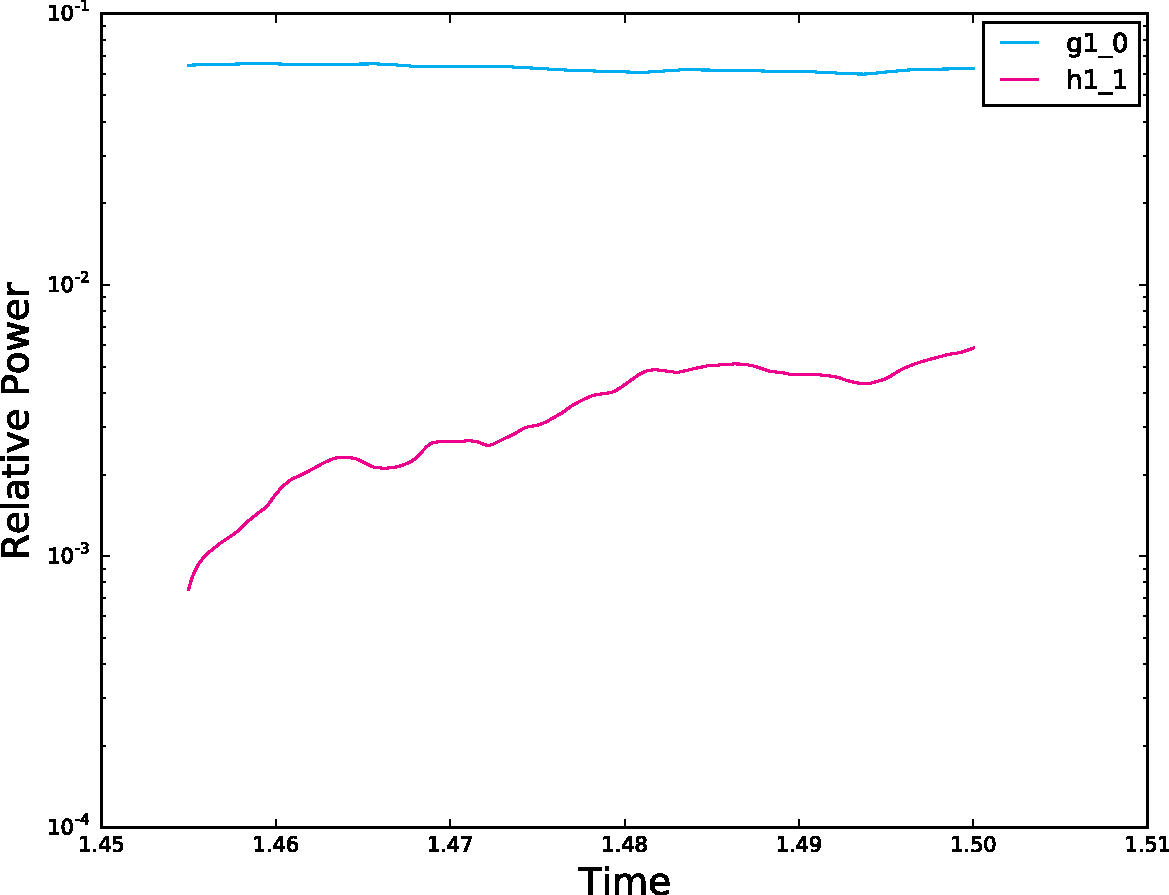
\includegraphics[width=0.8\textwidth]{gauss_coef_plot.pdf}
\caption{\small{Values of gauss coefficients $g^{0}_{1}$ and $h^{1}_{1}$ for model T\&B.D. plotted against model time (see secular variation discussion above).}}
\label{fig:source_gauss}
\end{figure}

\begin{figure}
\centering
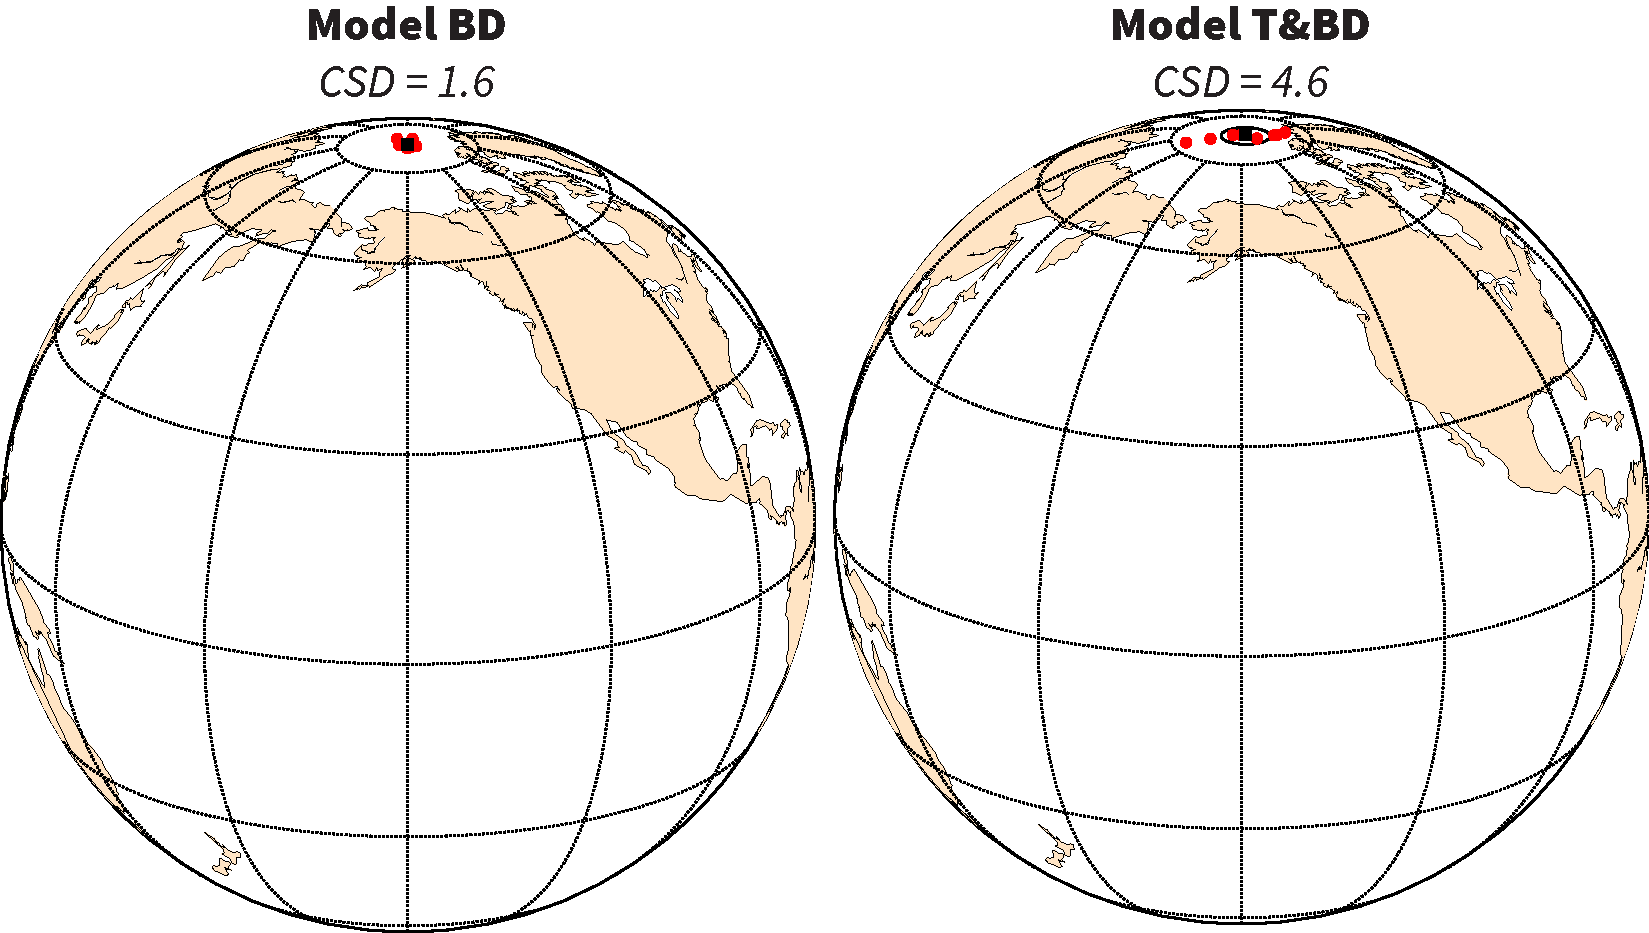
\includegraphics[width=\textwidth]{VGPS.pdf}
\caption{\small{Virtual geomagnetic poles and mean poles calculated from the magnetic field direction at 0\textdegree\ N, 0\textdegree\ E for each model. Virtual geomagnetic poles are plotted in red, with the mean pole and $A_{95}$ confidence ellipse plotted in black. The circular standard deviation (CSD)---one possible measure for the magnitude of secular variation---is labeled for each modelled pole distribution.}}
\label{fig:vgps}
\end{figure}



%\textbf{Outline}
%
%\begin{enumerate}
%\item{Introduction}
%    \begin{enumerate}
%    \item{The geomagnetic signature of inner core nucleation}
%        \begin{enumerate}
%        \item{Top-driven vs. bottom-driven geodynamo}
%        \end{enumerate}
%    \item{Modeling the geodynamo}
%    %Mainly Driscoll2016?
%    \end{enumerate}
%\item{Model parameters}
%\item{Results and Discussion}
%    \begin{enumerate}
%    \item{Future investigations}
%    \end{enumerate}
%\end{enumerate}

\clearpage

\footnotesize
\bibliographystyle{gsabull}
\bibliography{../../references/allrefs}

\end{document}

